\documentclass{beamer}
%\usepackage[all,arc,curve,frame,color]{xy}
%\usepackage{tkz-graph}
\usepackage{mathtools}
\usepackage{ragged2e,etoolbox}


\newenvironment{nstabbing}
  {\setlength{\topsep}{0pt}%
   \setlength{\partopsep}{0pt}%
   \tabbing}
  {\endtabbing}

\def\jump{ \quad \\ \vspace{0.7cm} \pause}
\newcommand{\nc}{\newcommand}
\nc{\pid}{\mathfrak{p} }
\nc{\dpid}{\delta_{\mathfrak{p}}}

\def\AA{{\mathbb A}}
\def\CC{{\mathbb C}}
\def\EE{{\mathcal E}}
\def\FF{{\mathcal F}}
\def\GG{{\mathcal G}}
\def\HH{{\mathcal H}}
\def\MM{{\mathcal M}}
\def\NN{{\mathbb N}}
\def\PP{{\mathbb P}}
\def\QQ{{\mathbb Q}}
\def\RR{{\mathbb R}}
\def\ZZ{{\mathbb Z}}
\def\aa{{\mathbf a}}
\def\bb{{\mathbf b}}
\def\del{\partial}
\def\kk{\Bbbk}
\def\mm{{\mathfrak m}}
\def\nn{{\mathfrak n}}
\def\pp{{\mathfrak p}}
\def\qq{{\mathfrak q}}
\def\rr{{\mathbf r}}
\def\uu{{\mathbf u}}
\def\vv{{\mathbf v}}
\def\ww{{\mathbf w}}
\def\xx{{\mathbf x}}
\def\yy{{\mathbf y}}
\def\zz{{\mathbf z}}
\newcommand{\PGL}{\textrm{PGL}}
\newcommand{\res}{\textrm{Res}}


\DeclareMathOperator{\Tail}{Tail}
\DeclareMathOperator{\Per}{Per}
\DeclareMathOperator{\PrePer}{PrePer}

\makeatletter
\def\th@mystyle{%
    \normalfont % body font
    \setbeamercolor{block title example}{bg=orange,fg=white}
    \setbeamercolor{block body example}{bg=orange!20,fg=black}
    \def\inserttheoremblockenv{exampleblock}
  }
\makeatother

\makeatletter
\def\th@thmstyle{%
    \normalfont % body font
    \setbeamercolor{block title example}{bg=blue,fg=white}
    \setbeamercolor{block body example}{bg=blue!20,fg=black}
    \def\inserttheoremblockenv{exampleblock}
  }
\makeatother

\definecolor{darkgreen}{RGB}{77,153,0}
\makeatletter
\def\th@qstnstyle{%
    \normalfont % body font
    \setbeamercolor{block title example}{bg=darkgreen,fg=white}
    \setbeamercolor{block body example}{bg=green!20,fg=black}
    \def\inserttheoremblockenv{exampleblock}
  }
\makeatother


\theoremstyle{thmstyle}
\newtheorem*{mythm}{Theorem}

\theoremstyle{mystyle}
\newtheorem*{remark}{Remark}
\newtheorem*{conjecture}{Conjecture}
\newtheorem*{mycor}{Corollary}
\newtheorem*{mylemma}{Lemma}

\theoremstyle{qstnstyle}
\newtheorem*{question}{Question}

\usepackage{remreset}% tiny package containing just the \@removefromreset command
\makeatletter
\@removefromreset{subsection}{section}
\makeatother
\setcounter{subsection}{1}

\newcommand\Wider[2][3em]{%
\makebox[\linewidth][c]{%
  \begin{minipage}{\dimexpr\textwidth+#1\relax}
  \raggedright#2
  \end{minipage}%
  }%
}

\mode<presentation>{\usetheme{CambridgeUS}\usecolortheme{dolphin}} 
%\setbeamertemplate{navigation symbols}{}
\setbeamertemplate{blocks}[rounded][shadow=false]


\title[Bounds for Preperiodic points]{Bound for preperiodic points for maps with good reduction}
%\subtitle[short subtitle]{long subtitle}
\author[S. Troncoso]{Sebastian Troncoso}
\institute[MSU]{Michigsn State University}
%\titlegraphic{\includegraphics[height=1.5cm]{../images/normale_pisa.png}}
\date[ January 04, 2017.]{ January 04, 2017. \\ \vspace{1cm} }


%\AtBeginSection[]{} % for optional outline or other recurrent slide
\AtBeginSection{\frame{\sectionpage}}
\begin{document}

\begin{frame}
\titlepage
\end{frame}

\begin{frame}
\frametitle{Notation}
Let $\phi:\mathbb{P}^n\to\mathbb{P}^n$ be a morphism. \\\quad\\
\pause
\textbf{orbit:} of a point $P\in\PP^n$: \quad \(P, \phi(P),
\phi^2(P),\phi^3(P),\ldots\)
\jump
\begin{nstabbing}
\textbf{Periodic point}: \= $\phi^n(P)=P$ for some $n\geq{1}$. \\
\> Minimal $n$ is called the \textbf{period} of $P$.
\end{nstabbing}
\jump
\textbf{Preperiodic point}: $\exists m\geq{0}$ such that $\phi^m(P)$
is periodic.
\pause
\vspace{2mm}

The set of $K$-rational preperiodic points is denoted by $Preper(\phi,K)$.


\jump
The \textbf{orbit length} of a preperiodic point $P$ is the cardinality of the orbit of $P$ (as a set).
\end{frame}

\begin{frame}
\frametitle{Tail points}

\textbf{Tail point}: A point that is preperiodic but not periodic.%.
\pause 


\begin{center}
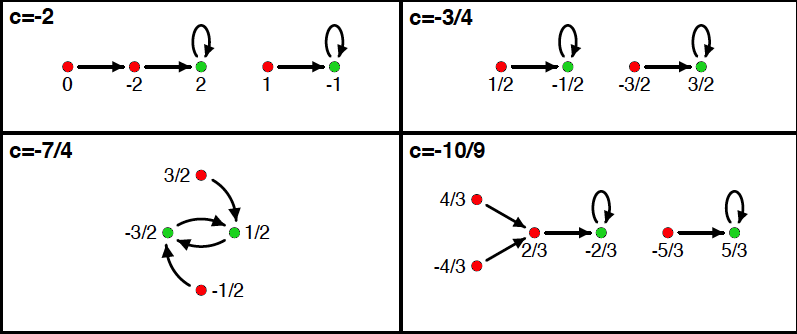
\includegraphics[width=1.0\linewidth]{placeholder4}
\end{center}

Tail points (red) and periodic point (green) of  $z^2+c$.
\end{frame}

\begin{frame}
\frametitle{Uniform boundedness of preperiodic points}
\begin{mythm}[Northcott 1950]
Let $\phi : \PP^n \to \PP^n$ be a morphism of degree $\geq{2}$
defined over a number field $K$. Then $\phi$ has
only finitely many preperiodic points in $\PP^n(K)$.
\end{mythm}

\quad\\

\pause

\begin{conjecture}[Uniform Boundedness Conjecture - Morton--Silverman
  1994]
There exists a bound $B = B(D,n,d)$ such that if $K/\mathbb{Q}$ is a number field of degree $D$, and $\phi:\mathbb{P}^n\rightarrow\mathbb{P}^n$ is a morphism of degree $d\geq{2}$ defined over $K$, then 
$$\#\text{PrePer}(\phi,K) \leq B.$$
%the number of $K$-preperiodic points of $f$ is less than or equal to $B$.
\end{conjecture}

\end{frame}


\begin{frame}

\textbf{GOAL:} Prove good bounds that depend additionally on the number of places of bad reduction of phi \pause (and sometimes don't depend on the degree!).


\end{frame}

\begin{frame}
\frametitle{Good reduction}

\begin{itemize}
\item For simplicity we will from now on deal only with rational maps $\phi:\mathbb{P}^1\to\mathbb{P}^1$. \pause
\item Let $K$ be a number field, $\mathcal{O}_K$ its ring of algebraic integers, $\mathfrak{p}$ a non zero prime ideal of $\mathcal{O}_K$
and $\mathcal{O}_{\mathfrak{p}}$ the local ring at $\pid$. \pause
\item Write $\phi$ in normal form: 
$$\phi([x : y]) = [F(x, y), G(x, y)],$$
where $F(x, y)$ and $G(x, y)$ are coprime
homogeneous polynomials of the same degree, with coefficients in $\mathcal{O}_\pid$ and at least one a $\pid$-unit. \pause
\item We say $\phi$ has \textbf{good reduction} at $\pid$ if $F$ and $G$ do not have a common zero module $\pid$ in $\mathbb{P}^1$.   \pause
\item In other words, $\phi$ does not drop degree mod $\pid$.  \pause
\item By convention, we say $\phi$ has bad reduction at all archimedean places.
\end{itemize}
\end{frame}

%\begin{frame}
%\frametitle{Bound on maximal period}
%\begin{mythm}[W.\ Narkiewicz 1988]
%Let $\phi \in K[z]$ be a polynomial of degree $\geq{2}$
%defined over a number field $K$ of degree $D=[K:\QQ]$. 
%Suppose $\phi$ has good reduction outside a finite set of places $S$, including all archimedean ones. Let $s=|S|$.
%\\\quad\\
%If $P$ is a $K$-rational periodic point of period $n$, then
%$$ n \leq (6\cdot 7^{D+2s})^\alpha,$$ where $\alpha=O(s\log{s}).$
%\end{mythm}
%\end{frame}




%\begin{frame}
%\frametitle{Bound on maximal orbit length of a preperiodic point}
%\begin{mythm}[J.K.\ Canci 2006]
%Let $\phi : \PP^1\to\PP^1$ be a rational map of degree at least two
%defined over a number field $K$. 
%Suppose $\phi$ has good reduction outside a finite set of places $S$, including all archimedean ones. Let $s=|S|$.
%\\\quad\\
%If $P\in\text{PrePer}(\phi,K)$ is of orbit length $n$, then
%$$n\leq\left[{e^{10}}^{12}(s+1)^8(log(5(s+1)))^8\right]^s.$$
%\end{mythm}
%\end{frame}

\begin{frame}
\frametitle{Bound on maximal orbit length of a preperiodic point }
\begin{mythm}[J.K.\ Canci, L.\ Paladino 2015]
Let $\phi : \PP^1\to\PP^1$ be a rational map of degree $\geq{2}$
defined over a number field $K$ and $[K, \mathbb{Q}]=D$. 
Suppose $\phi$ has good reduction outside a finite set of places $S$, including all archimedean ones. Let $s=|S|$.
If $P\in\text{PrePer}(\phi,K)$ is of orbit length $n$, then
$$n\leq \max\left\{(2^{16s-8}+3)\left[12s\log(5s)\right]^{D}, \left[12(s+2)\log(5s+5)\right]^{4D}\right\}
.$$
\end{mythm}
\end{frame}




%\begin{frame}
%\frametitle{From bound of maximal period to bound of $\#\text{Per}(\phi,K)$}
%
%\begin{remark}
%
%Given a bound on the maximal period of a $K$-rational periodic point, we can get a (naive) bound on the number of periodic points, as any periodic point of period $\leq{N}$ satisfies some equation $f^n(P)=P$ for $1\leq{n}\leq{N}$.
%
%\quad \\
%
%We can get in this way a bound that is on the order of $O(d^N)$, where $N$ is the maximal possible period.
%\end{remark}
%\end{frame}

%\begin{frame}
%\frametitle{Best \textbf{full} bound (so far) for polynomials}
%\begin{mythm}[R.L.\ Benedetto 2007]
%Let $\phi \in K[z]$ be a polynomial of degree $d\geq{2}$
%defined over a number field $K$ of degree $D=[K:\QQ]$. 
%Suppose $\phi$ has good reduction outside a finite set of places $S$, including all archimedean ones. Let $s=|S|$.
%The number of preperiodic points of $\phi$ in $\PP^1(K)$ is at most $O(s\log s)$ and $O(d^2/\log{d})$. 
%\end{mythm}
%
%\pause
%
%\begin{itemize}
%\item Proved by using nonarchimedean places $\nu$ of bad reduction and bounding the filled Julia set in the completion $K_\nu$.  \pause
%\item X.\ Faber (2015) used ``Benedetto's trick'' to find exact number of preperiodic points in certain infinite sequences of quadratic polynomials.
%\end{itemize}
%\end{frame}





\begin{frame}
\frametitle{Bounds independent of the degree}
\begin{mythm}[S.\ Troncoso 2016]
Let $K$ be a number field and $S$ a finite set of places of $K$ containing all the archimedean ones. Let $\phi $ be an endomorphism of $\PP^1$, defined over $K$, and $d \geq 2$ the degree of $\phi$. Assume $\phi$ has  good reduction outside $S$.
\begin{enumerate}

\item [(a)] \label{th 3 periodic}
If there are at least three $K$-rational tail points of $\phi$ then
$$|\Per(\phi,K)| \leq 2^{16|S|}+3. $$

\item [(b)] \label{th 4 preperiodic}
If there are at least four $K$-rational periodic points of $\phi$ then
$$|\Tail(\phi,K)| \leq 4(2^{16|S|}).$$
\end{enumerate}
\end{mythm}
\end{frame}

\begin{frame}
\frametitle{Bounds for Preperiodic points}
\begin{mythm}[S.\ Troncoso 2016]
Let $K$ be a number field and $S$ a finite set of places of $K$ containing all the archimedean ones. Let $\phi $ be an endomorphism of $\PP^1$, defined over $K$, and $d \geq 2$ the degree of $\phi$. Assume $\phi$ has  good reduction outside $S$. Then
\begin{enumerate}
\item [(a)] $|\Per(\phi,K)| \leq  2^{16|S|d^3}+3.$

\item [(b)] $|\Tail(\phi,K)| \leq  4(2^{16|S|d^3}) .$

\item [(c)] $|\PrePer(\phi,K)| \leq 5(2^{16|S|d^3})+3.$

\end{enumerate}
\end{mythm}
\end{frame}

\begin{frame}
\frametitle{Reciprocity of periodic and tail points}
\begin{mythm}[S.\ Troncoso 2016]
Let $\phi$ be an endomorphism of $\PP^1$, defined over $K$. Suppose $\phi$ has good reduction outside $S$. Let $R\in\PP^1(K)$ be a tail point and let $n$ be the period of the periodic part of the orbit of $R$. Let $P\in\PP^1(K)$ be any periodic point that is not $\phi^{mn}(R)$ for some $m$. Then $\delta_\pp(P,R)=0$ for every $\pp \notin S$.
\end{mythm}
\end{frame}

\begin{frame}
\frametitle{Techniques: $S$-unit equations}

\begin{itemize}
\item Almost every pair of $K$-rational tail point and $K$-rational periodic point induces $S$-unit equations. \pause
\item That means linear relations of the form $$au+bv=1$$  where  $(u,v) \in \left(\mathcal{O}_S^*\right)^2$ and $a,b\in{K}$. ($\mathcal{O}_S^{*}$ is the group of $S$-units) \pause
\item Beukers and Schlickewei's explicit bound on the number of solutions $(u,v) \in \left(\mathcal{O}_S^{*}\right)^2$ to the $S$-unit equation.\pause For $a,b\in{K}$ the number of solutions of $$au+bv=1$$ is bounded by $$2^{8(2|S|+2)}$$ \pause
\item The finitely many solutions to $au+bv=1$ give us a bound on $Per(\phi,K)$, $Tail(\phi,K)$ and $PrePer(\phi,K)$. 
\end{itemize}
\end{frame}


\begin{frame}
\frametitle{Parallel theorem by Canci and Vishkautsan}
\begin{mythm}[Canci, Vishkautsan  2016]
  Let $K$ be a number field and $S$ a finite set of places of $K$
  containing all the archimedean ones. Let
  $\phi\colon\PP^1\to\PP^1$ be rational map defined over $K$, where the degree $d$ of $\phi$ is $\geq 2$. Assume that 
  $\phi$ has good reduction outside $S$.  Then 
%the number of $K$-rational periodic points of the composition $\psi\circ\phi$ is bounded by 
$$\#\text{Per}(\phi, K) \leq \kappa d+\lambda,$$ 
where $\kappa=2^{2^5s}$ and $\lambda=2^{2^{77}s}$.
\end{mythm}
\end{frame}




%\begin{frame}
%\frametitle{$p$-adic chordal distance}
%
%Let $K$ be a number field, and $\nu$ a nonarchimedean place. 
%Let $P=[X_1:Y_1], Q=[X_2:Y_2] \in \PP^1(K)$. Then
%
%\quad \\ \pause
%\textbf{logarithmic $p$-adic chordal distance}:
%
%$$\delta_{\mathfrak{p}}\,(P,Q)=v_{\mathfrak{p}}\,(X_1Y_2-X_2Y_1)-\min\{v_{\mathfrak{p}}(X_1),v_{\mathfrak{p}}(Y_1)\}-\min\{v_{\mathfrak{p}}(X_2),v_{\mathfrak{p}}(Y_2)\}$$
%\end{frame}
%
%\begin{frame}
%\frametitle{$S$-integral points}
%
%\begin{itemize}
%\item Let $P,Q \in \PP^1(K)$. Then $P\equiv{Q}\pmod{\pid}$ iff $\delta_\pid(P,Q)\geq{1}$. \jump
%\item Let $S$ be a finite set of places of $K$ containing all the archimedean ones. \jump
%\item $P$ is \textbf{$S$-integral} with respect to $Q$ iff $\delta_\pid(P,Q)=0$ for all $\pid\not\in{S}$. \jump
%% \item A finite point $P$ is an $S$-integer iff it is $S$-integral with respect to $\infty$.
%\end{itemize}
%\end{frame}


\begin{frame}
\frametitle{Future directions: Preliminary results}
Joint work with J.K.\ Canci and S.\ Vishkautsan \\
\pause

\vspace{5mm}

The number of $K$-rational preperiodic points of rational functions with good reduction outside of $S$ is $O(d^2)$. 


\end{frame}

\begin{frame}
\frametitle{Future directions: Preliminary results (2)}

\begin{itemize}
\item The theorem on the reciprocity of periodic and tail points can be generalize in higher dimensions.
\pause

\item Reciprocity $K$-rational tail points and $K$-rational periodic hypersurface.

\pause

\item Similarly, we get a reciprocity $K$-rational tail hypersurface and $K$-rational periodic points.

\pause

\item With these theorems we can get similar consequences than the one dimensional case. However Hypotheses of general position are required. 

\pause

\item For instance, if $\Per_{\Phi}(H) \geq 2N+1$ and the hypersurfaces on the orbit of $H$ are in general position then $|Tail(\Phi,K)|$ is  bounded.
\end{itemize}


\end{frame}

\end{document}